\documentclass[main.tex]{subfiles}

\title{Inequalities}
\author{Senan Sekhon}
\date{July 17, 2025}
% Created July 17, 2025

\begin{document}

\maketitle

\section{Algebraic Inequalities}

\begin{proposition}\label{am_gm_inequality_2_numbers}
    Suppose $a,b\ge 0$. Then:
    \begin{equation*}
        \frac{a+b}{2} \ge \sqrt{ab}
    \end{equation*}
    Equality holds if and only if $a=b$.
\end{proposition}
\begin{proof}
    Since $0\le\qty(\sqrt{a}-\sqrt{b})^2=a-2\sqrt{ab}+b$, we have $\dfrac{a+b}{2}\ge\sqrt{ab}$. Equality holds if and only if $\sqrt{a}-\sqrt{b}=0$, i.e. $a=b$.
\end{proof}
\begin{proof}
    Consider the following diagram:
    \begin{center}
        \begin{tikzpicture}
            \draw (-3,0) arc (180:0:3);
            \fill (0,0) circle (2pt);
            \draw[fill=gray, fill opacity=0.1] (-3,0) -- (1,{sqrt(8)}) -- (1,0) -- cycle;
            \draw[fill=gray, fill opacity=0.2] (1,{sqrt(8)}) -- (1,0) -- (3,0) -- cycle;
            \draw (1,0) rectangle (0.75,0.25);
            \draw[latex-latex, very thick, red] (-3,0) -- (1,0) node[midway, below]{$a$};
            \draw[latex-latex, very thick, blue] (1,0) -- (3,0) node[midway, below]{$b$};
            \draw[thick, Green] (0,0) -- (0,3) node[pos=0.3, left]{$\dfrac{a+b}{2}$};
            \draw[thick, violet] (1,0) -- (1,{sqrt(8)}) node[pos=0.3, right]{$\sqrt{ab}$};
        \end{tikzpicture}
    \end{center}
    \vspace{-5pt}
    The \textcolor{Green}{green} line has length $\frac{a+b}{2}$ as it is the radius of a semicircle with diameter $a+b$. The \textcolor{violet}{violet} line has length $\sqrt{ab}$ as the two shaded triangles are similar. Since the \textcolor{Green}{green} line is longer than the \textcolor{violet}{violet} line (unless the two lines coincide), we have $\frac{a+b}{2}>\sqrt{ab}$ (unless $a=b$, in which case they are equal).
\end{proof}

\begin{theorem}[AM-GM Inequality]
    Suppose $a_1,a_2,\ldots,a_n\ge 0$. Then:
    \begin{equation}\label{am_gm_inequality_eq}
        \frac{a_1+a_2+\cdots+a_n}{n} \ge \sqrt[n]{a_1a_2\ldots a_n}
    \end{equation}
    Equality holds if and only if $a_1=a_2=\cdots=a_n$.
\end{theorem}
\begin{proof}
    Define $P(n)$ as the statement that \eqref{am_gm_inequality_eq} holds for $n\in\N$. Note that $P(1)$ holds trivially (since both sides reduce to $a_1$), and by \Cref{am_gm_inequality_2_numbers}, $P(2)$ also holds.\\
    
    We first show that $(P(m) \text{ and } P(2))\implies P(2m)$:
    \begin{align*}
        \frac{a_1+a_2+\cdots+a_{2m}}{2m}
        &= \frac{1}{2}\qty(\frac{a_1+a_2+\cdots+a_m}{m} + \frac{a_{m+1}+a_{m+2}+\cdots+a_{2m}}{m}) \\
        &\ge \frac{1}{2}\qty(\sqrt[m]{a_1a_2\ldots a_m} + \sqrt[m]{a_{m+1}a_{m+2}\ldots a_{2m}})
            \tag{by $P(m)$} \\
        &\ge \sqrt{\sqrt[m]{a_1a_2\ldots a_m}\sqrt[m]{a_{m+1}a_{m+2}\ldots a_{2m}}}
            \tag{by $P(2)$} \\
        &= \sqrt[2m]{a_1a_2\ldots a_{2m}}
    \end{align*}
    We now show that $P(m)\implies P(m-1)$. We will assume $a_1,a_2,\ldots,a_m$ are not all zero, otherwise $P(m-1)$ holds trivially. Define $a_m=\frac{a_1+a_2+\cdots+a_{m-1}}{m-1}$. Then we have:
    \begin{align*}
        \frac{a_1+a_2+\cdots+a_{m-1}+a_m}{m}
        &\ge \sqrt[m]{a_1a_2\ldots a_{m-1}a_m} \\
        \frac{a_1+a_2+\cdots+a_{m-1}+\frac{a_1+a_2+\cdots+a_{m-1}}{m-1}}{m}
        &\ge \sqrt[m]{a_1a_2\ldots a_{m-1}\qty(\frac{a_1+a_2+\cdots+a_{m-1}}{m-1})} \\
        \frac{a_1+a_2+\cdots+a_{m-1}}{m-1}
        &\ge \sqrt[m]{a_1a_2\ldots a_{m-1}}\qty(\frac{a_1+a_2+\cdots+a_{m-1}}{m-1})^{\tfrac{1}{m}} \\
        \qty(\frac{a_1+a_2+\cdots+a_{m-1}}{m-1})^{\tfrac{m-1}{m}}
        &\ge \sqrt[m]{a_1a_2\ldots a_{m-1}} \\
        \frac{a_1+a_2+\cdots+a_{m-1}}{m-1}
        &\ge \sqrt[m-1]{a_1a_2\ldots a_{m-1}} \\
    \end{align*}
    Thus $P(n)$ holds for all $n\in\N$.
\end{proof}

\begin{definition}
    Suppose $a_1,a_2,\ldots,a_n\ge0$ and $p\in\R\exc\{0\}$. The \textbf{$p$\textsuperscript{th} Hölder mean} of $a_1,a_2,\ldots,a_n$ is given by:
    \begin{equation*}
        M_p(a_1,a_2,\ldots,a_n)
        = \qty(\frac{a_1^p+a_2^p+\cdots+a_n^p}{n})^{\tfrac{1}{p}}
    \end{equation*}
\end{definition}

\begin{examples}\leavevmode
    \begin{itemize}
        \item If $p=1$, this is the \emph{arithmetic mean} $\dfrac{a_1+a_2+\cdots+a_n}{n}$.
        \item If $p=2$, this is the \emph{quadratic mean} (or \emph{root-mean-square}) $\sqrt{\dfrac{a_1^2+a_2^2+\cdots+a_n^2}{n}}$.
        \item If $p=-1$, this is the \emph{harmonic mean} $\dfrac{n}{\frac{1}{a_1}+\frac{1}{a_2}+\cdots+\frac{1}{a_n}}$.
    \end{itemize}
\end{examples}

\begin{proposition}\label{geometric_mean_is_0th_holder_mean}
    Suppose $a_1,a_2,\ldots,a_n\ge0$. Then $\lim_{p\to 0} M_p(a_1,a_2,\ldots,a_n)= \sqrt[n]{a_1a_2\cdots a_n}$.
\end{proposition}
\begin{proof}
    If $M_p(a_1,a_2,\ldots,a_n)=0$ for some $p\ne0$, then we must have $a_1=a_2= \cdots=a_n=0$. This implies that $M_p(a_1,a_2,\ldots,a_n)=0$ for all $p\ne0$, as well as $\sqrt[n]{a_1a_2\cdots a_n}=0$. Thus
    Note that:
    \begin{equation*}
        \log(M_p(a_1,a_2,\ldots,a_n))= \frac{1}{p}\log\qty(\frac{a_1^p+a_2^p+\cdots+a_n^p}{n})
    \end{equation*}
    By L'Hôpital's rule, we have:
    \begin{align*}
        \lim_{p\to 0} \log(M_p(a_1,a_2,\ldots,a_n))
        &= \lim_{p\to 0} \frac{\log\qty(\frac{a_1^p+a_2^p+\cdots+a_n^p}{n})}{p}
        = \lim_{p\to 0} \frac{\dv{p}\qty(\log\qty(\frac{a_1^p+a_2^p+\cdots+a_n^p}{n}))}{\dv{p}(p)} \\
        &= \lim_{p\to 0} \frac{\frac{n}{a_1^p+a_2^p+\cdots+a_n^p}\qty(\frac{a_1^p\log(a_1)+a_2^p\log(a_2)+\cdots+a_n^p\log(a_n)}{n})}{1} \\
        &= \lim_{p\to 0} \frac{a_1^p\log(a_1)+a_2^p\log(a_2)+\cdots+a_n^p\log(a_n)}{a_1^p+a_2^p+\cdots+a_n^p} \\
        &= \frac{1\cdot\log(a_1)+1\cdot\log(a_2)+\cdots+1\cdot\log(a_n)}{1+1+\cdots+1} \\
        &= \frac{\log(a_1)+\log(a_2)+\cdots+\log(a_n)}{n}
    \end{align*}
    Since the exponential function is continuous, we have:
    \begin{align*}
        \lim_{p\to 0} M_p(a_1,a_2,\ldots,a_n)
        &= \exp\qty(\lim_{p\to 0} \log(M_p(a_1,a_2,\ldots,a_n))) \\
        &= \exp\qty(\frac{\log(a_1)+\log(a_2)+\cdots+\log(a_n)}{n}) \\
        &= \exp\qty(\frac{1}{n}\log(a_1a_2\cdots a_n)) \\
        &= \sqrt[n]{a_1a_2\cdots a_n}
    \end{align*}
\end{proof}

\begin{proposition}
    Suppose $a_1,a_2,\ldots,a_n\ge 0$. Then:
    \begin{align*}
        \lim_{p\to-\infty} M_p(a_1,a_2,\ldots,a_n)= \min\{a_1,a_2,\ldots,a_n\} &&
        \lim_{p\to\infty} M_p(a_1,a_2,\ldots,a_n)= \max\{a_1,a_2,\ldots,a_n\}
    \end{align*}
\end{proposition}
\begin{proof}
    Assume without loss of generality that $a_1\ge a_2\ge\cdots\ge a_n$ (otherwise, rearrange $a_1,a_2,\ldots,a_n$). This implies that $\max\{a_1,a_2,\ldots,a_n\}=a_1$. We first rewrite $M_p(a_1,a_2,\ldots,a_n)$ as follows:
    \begin{align*}
        M_p(a_1,a_2,\ldots,a_n)
        &= \qty(\frac{a_1^p+a_2^p+\cdots+a_n^p}{n})^{1/p} \\
        &= \qty(\frac{a_1^p}{n}\qty(\qty(\frac{a_1}{a_1})^p+\qty(\frac{a_2}{a_1})^p+\cdots+\qty(\frac{a_n}{a_1})^p))^{1/p} \\
        &= \frac{a_1}{n^{1/p}}\qty(\qty(\frac{a_1}{a_1})^p+\qty(\frac{a_2}{a_1})^p+\cdots+\qty(\frac{a_n}{a_1})^p)^{1/p}
    \end{align*}
    Now define $f(p)= \qty(\frac{a_1}{a_1})^p+\qty(\frac{a_2}{a_1})^p+\cdots+\qty(\frac{a_n}{a_1})^p$. We can assume $p>0$ as we will eventually take the limit as $p\to\infty$. Since the first term is $1^p=1$, we have $f(p)\ge1$. Also, since $0\le a_k\le a_1$ for all $k=2,\ldots,n$, we have $0\le\qty(\frac{a_k}{a_1})^p\le1$. Thus $1\le f(p)\le n$ for all $p>0$, and so:
    \begin{equation*}
        \frac{a_1}{n^{1/p}}\le M_p(a_1,a_2,\ldots,a_n)\le a_1
    \end{equation*}
    Taking the limit as $p\to\infty$, we have:
    \begin{equation*}
        \lim_{p\to\infty} \frac{a_1}{n^{1/p}}\le\lim_{p\to\infty} M_p(a_1,a_2,\ldots,a_n)\le\lim_{p\to\infty} a_1
    \end{equation*}
    Since $\lim_{p\to\infty} n^{1/p}=1$, by the sandwich theorem, we have $\lim_{p\to\infty} M_p(a_1,a_2,\ldots,a_n)=a_1$. A similar proof shows that $\lim_{p\to-\infty} M_p(a_1,a_2,\ldots,a_n)=a_n$.
\end{proof}

\begin{lemma}\label{holder_geometric_mean_inequality}
    Suppose $a_1,a_2,\ldots,a_n\ge 0$ and $p>0$. Then:
    \begin{equation*}
        M_{-p}(a_1,a_2,\ldots,a_n)\le M_0(a_1,a_2,\ldots,a_n)\le M_p(a_1,a_2,\ldots,a_n)
    \end{equation*}
\end{lemma}
\begin{proof}
    Since the logarithm function $\log:(0,\infty)\to\R$ is concave, by Jensen's inequality, we have:
    \begin{align*}
        \log(\sqrt[p]{\prod_{k=1}^n a_k^p})
        = \frac{1}{n}\sumkn \log(a_k^p)
        \le \log(\frac{1}{n}\sumkn a_k^p)
    \end{align*}
    Taking exponentials of both sides yields:
    \begin{equation*}
        \sqrt[p]{\prod_{k=1}^n a_k^p}
        \le \frac{1}{n}\sumkn a_k^p
    \end{equation*}
    Raising both sides to the power $\frac{1}{p}$ yields:
    \begin{equation*}
        \prod_{k=1}^n a_k^p
        \le \qty(\frac{1}{n}\sumkn a_k^p)^{\tfrac{1}{p}}
    \end{equation*}
    Thus $M_0(a_1,a_2,\ldots,a_n)\le M_p(a_1,a_2,\ldots,a_n)$. Replacing $p$ with $-p$ in the above steps yields the other inequality (with the sign flipped, since $x^{-\tfrac{1}{p}}$ is a decreasing function).
\end{proof}

\begin{theorem}
    Suppose $a_1,a_2,\ldots,a_n\ge 0$ and $p,q\in\R$, $p<q$. Then $M_p(a_1,a_2,\ldots,a_n)\le M_q(a_1,a_2,\ldots,a_n)$.
\end{theorem}
\begin{proof}
    Suppose $0<p<q$ and define $f:[0,\infty)\to[0,\infty)$, $f(x)=x^{\frac{q}{p}}$. Then $f''(x)=\qty(\frac{q}{p})\qty(\frac{q}{p}-1)x^{\frac{q}{p}-1}$. Since $q>p$, we have $f''(x)\ge 0$ for all $x\in[0,\infty)$, so $f$ is convex. By Jensen's inequality, we have:
    \begin{equation*}
        \qty(\frac{1}{n}\sumkn a_k^p)^{\tfrac{q}{p}}
        = f\qty(\frac{1}{n}\sumkn a_k^p)
        \le \frac{1}{n}\sumkn f\qty(a_k^p)
        = \frac{1}{n}\sumkn a_k^q
    \end{equation*}
    Raising both sides to the power $\frac{1}{q}$, we get:
    \begin{equation*}
        \qty(\frac{1}{n}\sumkn a_k^p)^{\tfrac{1}{p}}
        = \qty(\frac{1}{n}\sumkn a_k^p)^{\tfrac{1}{q}}
    \end{equation*}
    Thus $M_p(a_1,a_2,\ldots,a_n)\le M_q(a_1,a_2,\ldots,a_n)$.\\

    Now suppose $p<q<0$. Repeating the above steps with $-q$ and $-p$ in place of $p$ and $q$ respectively yields the desired result.\\

    Now suppose $p<0<q$. By \Cref{holder_geometric_mean_inequality}, we have $M_p(a_1,a_2,\ldots,a_n)\le M_0(a_1,a_2,\ldots,a_n)\le M_q(a_1,a_2,\ldots,a_n)$.
\end{proof}

\begin{theorem}[Young's Inequality]
    Suppose $a,b\ge 0$ and $p,q>1$ such that $\frac{1}{p}+\frac{1}{q}=1$. Then:
    \begin{equation*}
        ab \le \frac{a^p}{p} + \frac{b^q}{q}
    \end{equation*}
    Equality holds if and only if $a^p=b^q$.
\end{theorem}
\begin{proof}
    Consider the following graphs:
    \begin{center}
        \newcommand*{\YoungsInequalityPlot}[3]{
            \draw[-latex, thick] (0,0) -- (4,0) node[right]{$x$};
            \draw[-latex, thick] (0,0) -- (0,4) node[above]{$y$};
            \fill[color=red!40, domain=0:{#1}] (0,0) -- plot ({\x},{f(\x)}) -- ({#1},0) node[below, color=red!40!black]{$a$} -- cycle;
            \fill[color=blue!40, domain=0:{g(#2)}] (0,0) -- plot ({\x},{f(\x)}) -- (0,{#2}) node[left, color=blue!40!black]{$b$} -- cycle;
            \draw[very thick, smooth, domain=0:4, samples=200] plot(\x,{f(\x)}) node[left]{$y=x^{p-1}$};
            \filldraw[very thick, violet, pattern=north west lines, pattern color=violet] (0,0) rectangle ({#1},{#2});
            \node[shape=ellipse, inner sep=1pt, fill=red!40] at (2.4,0.8) {$\dfrac{a^p}{p}$};
            \node[shape=ellipse, inner sep=1pt, fill=blue!40] at (1.3,2) {$\dfrac{b^q}{q}$};
            \node[font=\sffamily] at (2,-0.7) {#3};
        }
        \begin{tikzpicture}
            \pgfmathdeclarefunction{f}{1}{\pgfmathparse{1/2*(#1)^(3/2)}}
            \pgfmathdeclarefunction{g}{1}{\pgfmathparse{(2*#1)^(2/3)}} % Inverse of f
            \begin{scope}[shift={(-5,0)}]
                \YoungsInequalityPlot{3.6}{3}{Case 1: $b<a^{p-1}$}
            \end{scope}
            \begin{scope}[shift={(0,0)}]
                \YoungsInequalityPlot{(6.4)^(2/3)}{3.2}{Case 2: $b=a^{p-1}$}
            \end{scope}
            \begin{scope}[shift={(5,0)}]
                \YoungsInequalityPlot{3}{3.4}{Case 3: $b>a^{p-1}$}
            \end{scope}
        \end{tikzpicture}
    \end{center}
    In all cases, the area of the hatched rectangle is $ab$, while the sum of the red and blue areas is $\frac{a^p}{p}+\frac{b^q}{q}$. Thus $ab\le\frac{a^p}{p}+\frac{b^q}{q}$, and equality holds only in case 2 ($a^p=b^q$).
\end{proof}
\begin{proof}[Alternative Proof]
    Define $f:[0,\infty)\to\R$, $f(x)=\frac{x^p}{p}+\frac{b^q}{q}-bx$. We want to show that $f(x)\ge 0$ for all $x\in[0,\infty)$. Differentiating yields $f'(x)=x^{p-1}-b$, which is zero if and only if $x^{p-1}=b$, i.e. $x=b^{q-1}$ (since $(p-1)(q-1)=1$). We also have:
    \begin{align*}
        f\qty(b^{q-1})
        = \frac{b^{p(q-1)}}{p}+\frac{b^q}{q}-b^q
        = \frac{b^q}{p} + \frac{b^q}{q} - b^q
        = 0
        &&
        f''\qty(b^{q-1})
        = (p-1)b^{(p-2)(q-1)}
        > 0
    \end{align*}
    Thus $f(x)\ge 0$ for all $x\in[0,\infty)$, and $f(x)=0$ if and only if $x=b^{q-1}$. 
\end{proof}

\begin{theorem}[Hölder's Inequality]
    Suppose $a_1,a_2,\ldots,a_,b_1,b_2,\ldots,b_n\ge 0$, $p,q>1$ and $\frac{1}{p}+\frac{1}{q}=1$. Then:
    \begin{equation}\label{holder_inequality_eq}
        \sumkn a_kb_k \le \qty(\sumkn a_k^p)^{\tfrac{1}{p}}\qty(\sumkn b_k^q)^{\tfrac{1}{q}}
    \end{equation}
    Equality holds if and only if $\qty(a_1,a_2,\ldots,a_n)$ and $\qty(b_1,b_2,\ldots,b_n)$ are proportional.
\end{theorem}

\begin{theorem}[Minkowski's Inequality]
    Suppose $a_1,a_2,\ldots,a_,b_1,b_2,\ldots,b_n\in\C$, $p,q>1$ and $\frac{1}{p}+\frac{1}{q}=1$. Then:
    \begin{equation}\label{minkowski_inequality_eq}
        \qty(\sumkn \abs{a_k+b_k})^{\tfrac{1}{p}} \le \qty(\sumkn \abs{a_k}^p)^{\tfrac{1}{p}} + \qty(\sumkn \abs{b_k}^p)^{\tfrac{1}{p}}
    \end{equation}
    Equality holds if and only if $\qty(a_1,a_2,\ldots,a_n)$ and $\qty(b_1,b_2,\ldots,b_n)$ are positively proportional.
\end{theorem}

\begin{theorem}[Hardy's Inequality]\label{hardyseq}
    Suppose $(a_n)$ is a sequence of non-negative numbers. Then for all $p>1$, we have:
    \begin{equation*}
        \sumn\qty(\frac{a_1+a_2+\cdots+a_n}{n})^p\le\qty(\frac{p}{p-1})^p\sumn a_n^p
    \end{equation*}
    If the right side is finite, equality holds if and only if $a_n=0$ for all $n\in\N$.
\end{theorem}
\begin{proof}
    For each $n\in\N$, define $s_n= \frac{a_1+a_2+\cdots+a_n}{n}$ and $b_n=s_n^{p-1}$. By Hölder's inequality, we have:
    \begin{equation*}
        \sumn a_nb_n\le\qty(\sumn a_n^p)^{\tfrac{1}{p}}\qty(\sumn b_n^q)^{\tfrac{1}{q}}
    \end{equation*}
    Where $\frac{1}{p}+\frac{1}{q}=1$. Since $\frac{1}{q}= \frac{p-1}{p}$ and $b_n^q=s_n^{(p-1)q}=s_n^p$, this reduces to:
    \begin{equation}\label{hardyseq:1}
        \sumn a_ns_n^{p-1}\le\qty(\sumn a_n^p)^{\tfrac{1}{p}}\qty(\sumn s_n^p)^{\tfrac{p-1}{p}}
    \end{equation}
    Note that for each $n\in\N$, we have $ns_n-(n-1)s_{n-1}=a_n$ (provided we define $s_0=0$). This yields:
    \begin{equation*}
        \sumn a_ns_n^{p-1}= \sumn s_n^{p-1}(ns_n-(n-1)s_{n-1})= \sumn ns_n^p-\sumn (n-1)s_n^{p-1}s_{n-1}
    \end{equation*}
    By Young's inequality, we have $s_n^{p-1}s_{n-1}\le\frac{s_{n-1}^p}{p}+\frac{(p-1)s_n^p}{p}$. Thus:
    \begin{align*}
        \sumn a_ns_n^{p-1}
        &\ge\sumn ns_n^p-\sumn (n-1)\qty(\frac{s_{n-1}^p}{p}+\frac{(p-1)s_n^p}{p}) \\
        &= \sumn ns_n^p-\frac{1}{p}\sumn (n-1)s_{n-1}^p-\frac{p-1}{p}\sumn (n-1)s_n^p
    \end{align*}
    We can rewrite the middle term as $\sumn (n-1)s_{n-1}^p= \sumn[0] ns_n^p= \sumn s_n^p$. This yields:
    \begin{align}\label{hardyseq:2}
        \sumn a_ns_n^{p-1}
        &\ge\sumn ns_n^p-\frac{1}{p}\sumn ns_n^p-\frac{p-1}{p}\sumn (n-1)s_n^p \nonumber\\
        &= \frac{p-1}{p}\sumn ns_n^p-\frac{p-1}{p}\sumn (n-1)s_n^p
        = \frac{p-1}{p}\sumn s_n^p
    \end{align}
    Combining \eqref{hardyseq:1} and \eqref{hardyseq:2}, we get:
    \begin{equation*}
        \frac{p-1}{p}\sumn s_n^p\le\qty(\sumn a_n^p)^{\tfrac{1}{p}}\qty(\sumn s_n^p)^{\tfrac{p-1}{p}}
    \end{equation*}
    Rearranging yields:
    \begin{equation*}
        \sumn s_n^p\le\qty(\frac{p}{p-1})^p\sumn a_n^p
    \end{equation*}
    % https://math.stackexchange.com/questions/3956889/prove-sum-k-1n-left-fraca-1a-2-cdots-a-kk-rightp-left-frac?noredirect=1&lq=1
\end{proof}

\begin{theorem}[Carleman's Inequality]\label{carleman_inequality}
    Suppose $(a_n)$ is a sequence of non-negative numbers. Then:
    \begin{equation*}
        \sumn\sqrt[n]{a_1a_2\cdots a_n}\le e\sumn a_n
    \end{equation*}
\end{theorem}
\begin{proof}
    Suppose $n\in\N$. Applying the AM-GM inequality to $1a_1,2a_2,\ldots,na_n$, we get:
    \begin{equation*}
        \frac{1a_1+2a_2+\cdots+na_n}{n}\ge\sqrt[n]{(1a_1)(2a_2)\cdots(na_n)}=(n!)^{1/n}\cdot\sqrt[n]{a_1a_2\cdots a_n}
    \end{equation*}
    By Stirling's inequality, we have $(n+1)!\ge\sqrt{2\pi(n+1)}\qty(\frac{n+1}{e})^{n+1}$. This yields:
    \begin{equation*}
        n!= \frac{(n+1)!}{n+1}\ge\frac{1}{n+1}\sqrt{2\pi(n+1)}\qty(\frac{n+1}{e})^{n+1}= \frac{\sqrt{2\pi(n+1)}}{e}\qty(\frac{n+1}{e})^n\ge\qty(\frac{n+1}{e})^n
    \end{equation*}
    Thus $(n!)^{-1/n}\le\frac{e}{n+1}$. We now have:
    \begin{equation*}
        \sqrt[n]{a_1a_2\cdots a_n}\le(n!)^{-1/n}\frac{1a_1+2a_2+\cdots+na_n}{n}\le e\frac{1a_1+2a_2+\cdots+na_n}{n(n+1)}
    \end{equation*}
    Summing the expression on the right from $n=1$ to $\infty$, we get:
    \begin{align*}
        \sumn\frac{1a_1+2a_2+\cdots+na_n}{n(n+1)}
        = \sumn\frac{1}{n(n+1)}\sumkn ka_k= \sumk ka_k\sumn[k] \frac{1}{n(n+1)}
        = \sumk ka_k\frac{1}{k}
        = \sumk a_k
    \end{align*}
    Thus, we have:
    \begin{equation*}
        \sumn\sqrt[n]{a_1a_2\cdots a_n}\le e\sumn a_n
    \end{equation*}
    % \remind{CLEAN UP THIS PROOF!!!}
    % https://en.wikipedia.org/wiki/Carleman%27s_inequality#Proof
\end{proof}
\begin{proof}[Alternative Proof (using Hardy's inequality)]
    Applying Hardy's inequality to the sequence $\qty(a_n^{1/p})$, we have:
    \begin{equation*}
        \sumn\qty(\frac{a_1^{1/p}+a_2^{1/p}+\cdots+a_n^{1/p}}{n})^p\le\qty(\frac{p}{p-1})^p\sumn a_n
    \end{equation*}
    We now take the limit of both sides as $p\to\infty$. By \Cref{geometric_mean_is_0th_holder_mean}, we have:
    \begin{equation*}
        \lim_{p\to\infty} \qty(\frac{a_1^{1/p}+a_2^{1/p}+\cdots+a_n^{1/p}}{n})^p
        = \sqrt[n]{a_1a_2\cdots a_n}
    \end{equation*}
    Since $\lim_{p\to\infty} \qty(\frac{p}{p-1})^p=e$, we get:
    \begin{equation*}
        \sumn\sqrt[n]{a_1a_2\cdots a_n}\le e\sumn a_n
    \end{equation*}
    % https://en.wikipedia.org/wiki/Carleman%27s_inequality#Proof
\end{proof}

The following example shows that the constant $e$ in \hyperref[carleman_inequality]{Carleman's inequality} is optimal, it cannot be replaced with a smaller number.

\begin{example}
    Suppose $N\in\N$ and $a_n= \begin{cases} \frac{1}{n} & n\le N \\ 0 & n>N \end{cases}$. Then we have:
    \begin{align}\label{carleman_inequality_optimal_1}
        \sumn\sqrt[n]{a_1a_2\cdots a_n}
        &= \sum_{n=1}^N \sqrt[n]{\frac{1}{1}\cdot\frac{1}{2}\cdots\frac{1}{n}}
        = \sum_{n=1}^N \sqrt[n]{\frac{1}{n!}}
        = \sum_{n=1}^N (n!)^{-1/n}\\
        \label{carleman_inequality_optimal_2}
        \sumn a_n
        &= \sum_{n=1}^N \frac{1}{n}
    \end{align}
    By Stirling's inequality, for all $n\in\N$, we have $n!\le\sqrt{2\pi n}\qty(\frac{n}{e})^ne^{\frac{1}{12n}}$, and so $(n!)^{-1/n}\ge(2\pi n)^{-\frac{1}{2n}}\qty(\frac{e}{n})e^{-\frac{1}{12n^2}}$. Since $\limn(2\pi n)^{-\frac{1}{2n}}= \limn e^{-\frac{1}{12n^2}}=1$, for any $a<1$, there exists $N\in\N$ such that $(2\pi n)^{-\frac{1}{2n}}e^{-\frac{1}{12n^2}}>a$ for all $n\ge N$. Thus \eqref{carleman_inequality_optimal_2} can be made arbitrarily close to \eqref{carleman_inequality_optimal_1}.
\end{example}

To achieve equality, we must have $1a_1=2a_2=\cdots=na_n$ for all $n\in\N$, i.e. $a_n=\frac{c}{n}$ for all $n\in\N$, where $c\ge 0$ is some constant. However, since the harmonic series $\sumn\frac{1}{n}$ diverges, we cannot get both sides to be equal to a finite value (unless $c=0$). Thus while the constant $e$ in \hyperref[carleman_inequality]{Carleman's inequality} is optimal, it is never attained non-trivially, i.e. unless both sides are $0$ or both sides are $\infty$.

\section{Integral Inequalities}

\begin{definition}
    Suppose $(X,\As,\mu)$ is a finite measure space, $f\in\Ms^+(X)$ and $p\in\R\exc\{0\}$. The \textbf{$p$\textsuperscript{th} Hölder mean} of $f$ is given by:
    \begin{equation*}
        M_p(f)= \qty(\frac{1}{\mu(X)}\int f^p\dmu)^{1/p}
    \end{equation*}
\end{definition}

\begin{proposition}\label{geometric_mean_is_0th_holder_mean_for_integrals}
    Suppose $f\ge0$. Then $\lim_{p\to 0} M_p(f)= \exp\qty(\frac{1}{\mu(X)}\int \log(f)\dmu)$.
\end{proposition}
\begin{proof}
    If $M_p(f)=0$ for some $p\ne0$, then we must have $a_1=a_2= \cdots=a_n=0$. This implies that $M_p(a_1,a_2,\ldots,a_n)=0$ for all $p\ne0$, as well as $\sqrt[n]{a_1a_2\cdots a_n}=0$. Thus
    Note that:
    \begin{equation*}
        \log(M_p(f))= \frac{1}{p}\log\qty(\frac{1}{\mu(X)}\int f^p\dmu)
    \end{equation*}
    By L'Hôpital's rule, we have:
    \begin{align*}
        \lim_{p\to 0} \log(M_p(f))
        &= \lim_{p\to 0} \frac{\log\qty(\frac{1}{\mu(X)}\int f^p\dmu)}{p}
        = \lim_{p\to 0} \frac{\dv{p}\qty(\log\qty(\frac{1}{\mu(X)}\int f^p\dmu))}{\dv{p}(p)}
        = \lim_{p\to 0} \frac{\frac{\mu(X)}{\int f^p\dmu}\qty(\frac{\int f^p\log(f)\dmu}{\mu(X)})}{1} \\
        &= \lim_{p\to 0} \frac{\int f^p\log(f)\dmu}{\int f^p\dmu}
        = \frac{\int\log(f)\dmu}{\int 1\dmu}
        = \frac{\int\log(f)\dmu}{\mu(X)}
    \end{align*}
    Since the exponential function is continuous, we have:
    \begin{align*}
        \lim_{p\to 0} M_p(f)
        = \exp\qty(\lim_{p\to 0} \log(M_p(f)))
        = \exp\qty(\frac{1}{\mu(X)}\int\log(f)\dmu)
    \end{align*}
\end{proof}

\begin{theorem}[Hardy's Inequality for Integrals]\label{hardys_inequality_for_integrals}
    Suppose $f\in\Ms^+((0,\infty))$ and $p>1$. Then:
    \begin{equation*}
        \int_0^\infty \qty(\frac{1}{x}\int_0^x f(t)\dt)^p\dx
        \le \qty(\frac{p}{p-1})^p\int_0^\infty f(x)^p\dx
    \end{equation*}
\end{theorem}
\begin{proof}
    We first substitute $t=sx$ in the inner integral on the left side:
    \begin{equation*}
        \int_0^\infty \qty(\frac{1}{x}\int_0^x f(t)\dt)^p\dx
        = \int_0^\infty \qty(\int_0^1 f(sx)\ds)^p\dx
    \end{equation*}
    By \hyperref[minkowskis_inequality_for_integrals]{Minkowski's inequality for integrals}, we have:
    \begin{equation*}
        \qty(\int_0^\infty \qty(\int_0^1 f(sx)\ds)^p\dx)^{1/p}
        \le \int_0^1 \qty(\int_0^\infty f(sx)^p\dx)^{1/p}\ds
    \end{equation*}
    Switching back to $sx=t$ in the inner integral, we get:
    \begin{equation*}
        \int_0^1 \qty(\int_0^\infty f(sx)^p\dx)^{1/p}\ds
        = \int_0^1 s^{-1/p}\qty(\int_0^\infty f(t)^p\dt)^{1/p}\ds
        = \frac{p}{p-1}\qty(\int_0^\infty f(t)^p\dt)^{1/p}
    \end{equation*}
    Thus:
    \begin{equation*}
        \int_0^\infty \qty(\frac{1}{x}\int_0^x f(t)\dt)^p\dx
        \le \qty(\frac{p}{p-1})^p\int_0^\infty f(x)^p\dx
    \end{equation*}
    % https://en.wikipedia.org/wiki/Hardy%27s_inequality#Proof_of_the_inequality
\end{proof}

\begin{theorem}[Carleman's Inequality for Integrals]
    Suppose $f\in\Ms^+((0,\infty))$. Then:
    \begin{equation*}
        \int_0^\infty \exp\qty(\frac{1}{x}\int_0^x \log(f(t))\dt)\dx
        \le e\int_0^\infty f(x)\dx
    \end{equation*}
\end{theorem}
\begin{proof}
    Applying \hyperref[hardys_inequality_for_integrals]{Hardy's inequality for integrals} to $f^{1/p}$, we have:
    \begin{equation*}
        \int_0^\infty \qty(\frac{1}{x}\int_0^x f(t)^{1/p}\dt)^p\dx
        \le\qty(\frac{p}{p-1})^p\int_0^\infty f(x)\dx
    \end{equation*}
    We now take the limit of both sides as $p\to\infty$. By \Cref{geometric_mean_is_0th_holder_mean_for_integrals}, we have
    \begin{equation*}
        \lim_{p\to\infty} \qty(\frac{1}{x}\int_0^x f(t)^{1/p}\dt)^p
        = \exp\qty(\frac{1}{x}\int_0^x \log(f(t))\dt)
    \end{equation*}
    Since $\lim_{p\to\infty} \qty(\frac{p}{p-1})^p=e$, we get:
    \begin{equation*}
        \int_0^\infty \exp\qty(\frac{1}{x}\int_0^x \log(f(t))\dt)\dx
        \le e\int_0^\infty f(x)\dx
    \end{equation*}
\end{proof}

\begin{theorem}[Miknowski's Inequality for Integrals]\label{minkowskis_inequality_for_integrals}
    Suppose $(X,\As,\mu)$ and $(Y,\Bs,\nu)$ are $\sigma$-finite measure spaces and $f\in\Ms^+(X\times Y,\As\otimes\Bs)$. Then:
    \begin{equation*}
        \qty(\int_X \qty(\int_Y f(x,y)\dnu(y))^p\dmu(x))^{1/p}
        \le \int_Y \qty(\int_X f(x,y)^p\dmu(x))^{1/p}\dnu(y)
    \end{equation*}
    % Folland Theorem 6.19 (Page 194)
\end{theorem}
\begin{proof}
    Define $g\in\Ms^+(X,\As)$ by $g(x)= \int_Y f(x,y)\dnu(y)$. Suppose $\int_X g(x)^p\dmu(x)<\infty$ (we do not need to assume $(X,\As,\mu)$ or $(Y,\Bs,\nu)$ is finite). Then we have:
    \begin{align*}
        \int_X g(x)^p\dmu(x)
        &= \int_X g(x)^{p-1}g(x)\dmu(x) \\
        &= \int_X \int_Y f(x,y)g(x)^{p-1}\dnu(y)\dmu(x) \\
        &= \int_Y \int_X f(x,y)g(x)^{p-1}\dnu(y)\dmu(x) \tag{by Tonelli's theorem} \\
        &= \int_Y \qty(\int_X f(x,y)^p\dmu(x))^{\tfrac{1}{p}} \qty(\int_X g(x)^{p}\dmu(x))^{\tfrac{p-1}{p}}\dnu(y) \tag{by Hölder's inequality} \\
        &= \qty(\int_X g(x)^{p}\dmu(x))^{\tfrac{p-1}{p}} \int_Y \qty(\int_X f(x,y)^p\dmu(x))^{\tfrac{1}{p}}\dnu(y)
    \end{align*}
    Dividing through by $\qty(\int_X g(x)^{p}\dmu(x))^{\tfrac{p-1}{p}}$, we get:
    \begin{equation*}
        \qty(\int_X g(x)^{p}\dmu(x))^{\tfrac{1}{p}}
        = \int_Y \qty(\int_X f(x,y)^p\dmu(x))^{\tfrac{1}{p}}\dnu(y)
    \end{equation*}
    Which is the desired result.\\
    
    Now suppose $\int_X g(x)^p\dmu(x)= \infty$. Since $(X,\As,\mu)$ and $(Y,\Bs,\nu)$ are $\sigma$-finite, there are increasing sequences of sets $(A_m)_{m=1}^\infty$ in $\As$ and $(B_n)_{n=1}^\infty$ in $\Bs$ such that $\mu(A_m)<\infty$ for all $m\in\N$, $\nu(B_n)<\infty$ for all $n\in\N$, $\cuppm A_m=X$ and $\cuppn B_n=Y$. For each $k\in\N$, define $f_k\in\Ms^+(X\times Y,\As\otimes\Bs)$ by $f_k(x,y)= \min\{f(x,y),k\}$. Then for all $k,m,n\in\N$, we have:
    \begin{equation*}
        \qty(\int_{A_m} \qty(\int_{B_n} f_k(x,y)\dnu(y))^p\dmu(x))^{1/p}
        \le \int_{B_n} \qty(\int_{A_m} f_k(x,y)^p\dmu(x))^{1/p}\dnu(y)
    \end{equation*}
    Taking the limit as $k\to\infty$, then $m\to\infty$ and $n\to\infty$ and using the monotone convergence theorem each time yields the desired result.
    % https://math.stackexchange.com/a/3738061
\end{proof}






\end{document}